% Options for packages loaded elsewhere
\PassOptionsToPackage{unicode}{hyperref}
\PassOptionsToPackage{hyphens}{url}
\PassOptionsToPackage{dvipsnames,svgnames,x11names}{xcolor}
\documentclass[
  british,
  11pt,
  a4paper,
]{article}
\usepackage{xcolor}
\usepackage[margin=25mm]{geometry}
\usepackage{amsmath,amssymb}
\setcounter{secnumdepth}{-\maxdimen} % remove section numbering
\usepackage{iftex}
\ifPDFTeX
  \usepackage[T1]{fontenc}
  \usepackage[utf8]{inputenc}
  \usepackage{textcomp} % provide euro and other symbols
\else % if luatex or xetex
  \usepackage{unicode-math} % this also loads fontspec
  \defaultfontfeatures{Scale=MatchLowercase}
  \defaultfontfeatures[\rmfamily]{Ligatures=TeX,Scale=1}
\fi
\usepackage{lmodern}
\ifPDFTeX\else
  % xetex/luatex font selection
\fi
% Use upquote if available, for straight quotes in verbatim environments
\IfFileExists{upquote.sty}{\usepackage{upquote}}{}
\IfFileExists{microtype.sty}{% use microtype if available
  \usepackage[]{microtype}
  \UseMicrotypeSet[protrusion]{basicmath} % disable protrusion for tt fonts
}{}
\makeatletter
\@ifundefined{KOMAClassName}{% if non-KOMA class
  \IfFileExists{parskip.sty}{%
    \usepackage{parskip}
  }{% else
    \setlength{\parindent}{0pt}
    \setlength{\parskip}{6pt plus 2pt minus 1pt}}
}{% if KOMA class
  \KOMAoptions{parskip=half}}
\makeatother
\usepackage{longtable,booktabs,array}
\newcounter{none} % for unnumbered tables
\usepackage{calc} % for calculating minipage widths
% Correct order of tables after \paragraph or \subparagraph
\usepackage{etoolbox}
\makeatletter
\patchcmd\longtable{\par}{\if@noskipsec\mbox{}\fi\par}{}{}
\makeatother
% Allow footnotes in longtable head/foot
\IfFileExists{footnotehyper.sty}{\usepackage{footnotehyper}}{\usepackage{footnote}}
\makesavenoteenv{longtable}
\usepackage{graphicx}
\makeatletter
\newsavebox\pandoc@box
\newcommand*\pandocbounded[1]{% scales image to fit in text height/width
  \sbox\pandoc@box{#1}%
  \Gscale@div\@tempa{\textheight}{\dimexpr\ht\pandoc@box+\dp\pandoc@box\relax}%
  \Gscale@div\@tempb{\linewidth}{\wd\pandoc@box}%
  \ifdim\@tempb\p@<\@tempa\p@\let\@tempa\@tempb\fi% select the smaller of both
  \ifdim\@tempa\p@<\p@\scalebox{\@tempa}{\usebox\pandoc@box}%
  \else\usebox{\pandoc@box}%
  \fi%
}
% Set default figure placement to htbp
\def\fps@figure{htbp}
\makeatother
\ifLuaTeX
\usepackage[bidi=basic,shorthands=off]{babel}
\else
\usepackage[bidi=default,shorthands=off]{babel}
\fi
\ifLuaTeX
  \usepackage{selnolig} % disable illegal ligatures
\fi
\setlength{\emergencystretch}{3em} % prevent overfull lines
\providecommand{\tightlist}{%
  \setlength{\itemsep}{0pt}\setlength{\parskip}{0pt}}
\usepackage[authoryear,round]{natbib}
\bibliographystyle{plainnat}
\usepackage{amsmath,amssymb,mathtools}
\usepackage[T1]{fontenc}
\usepackage{microtype}
\usepackage{float}
\floatplacement{figure}{H}
\newcommand{\atanh}{\operatorname{atanh}}
\newcommand{\sech}{\operatorname{sech}}
\newcommand{\diam}{\operatorname{diam}}
\newcommand{\SW}{\operatorname{SW}}
\newcommand{\GHSW}{\operatorname{GHSW}}
\newcommand{\TV}{\operatorname{TV}}
\newcommand{\sgn}{\operatorname{sgn}}
\usepackage{bookmark}
\IfFileExists{xurl.sty}{\usepackage{xurl}}{} % add URL line breaks if available
\urlstyle{same}
\hypersetup{
  pdftitle={Compact completion and uniform statistical bounds for hyperbolic geodesic sliced Wasserstein distance},
  pdfauthor={Anonymous},
  pdflang={en-GB},
  colorlinks=true,
  linkcolor={black},
  filecolor={Maroon},
  citecolor={teal},
  urlcolor={teal},
  pdfcreator={LaTeX via pandoc}}

\title{Compact completion and uniform statistical bounds for hyperbolic
geodesic sliced Wasserstein distance}
\usepackage{etoolbox}
\makeatletter
\providecommand{\subtitle}[1]{% add subtitle to \maketitle
  \apptocmd{\@title}{\par {\large #1 \par}}{}{}
}
\makeatother
\subtitle{Exact boundary geometry in every dimension, a correction, and
a complete radial augmentation}
\author{Anonymous}
\date{4 November 2026 (version 0.1.0-candidate; unrefereed)}

\begin{document}
\maketitle

{
\setcounter{tocdepth}{2}
\tableofcontents
}
\clearpage

\section{Abstract}\label{abstract}

Geodesic hyperbolic sliced Wasserstein distance is a cheap way to
compare probability distributions on hyperbolic space, used for data
embedded in hyperbolic geometry. We determine exactly what this distance
measures. For real hyperbolic space of dimension \(d\geq2\) and every
\(1\leq p<\infty\), it extends to a finite metric on all probability
measures, with no moment assumption. Its metric completion is the space
of probability measures on the closed Klein ball, and it metrises the
weak topology there. Its exact diameter is \(2C_{d,p}^{1/p}\), where
\(C_{d,p}\) is the \(p\)th absolute moment of the density
\(c_d\operatorname{sech}^{d-1}t\). Consequently it controls ordinary
weak convergence but not hyperbolic transport moments, and it is
exponentially insensitive to how deep points lie towards infinity. We
give the three exact radial rates of approach to the ideal boundary, and
the metric that the distance induces on the boundary sphere in every
dimension: a square-root snowflake of the angle when \(d=2\), a
logarithmically corrected angle when \(d=3\), and a metric bi-Lipschitz
to the angle when \(d\geq4\). We give a counterexample to the
vanishing-at-infinity assertion in Proposition 19 of Bonet, Drumetz and
Courty (Journal of Machine Learning Research, 2025). We prove
distribution-free \(n^{-1/2}\) minimax rates for the powered loss, the
matching \(n^{-1/(2p)}\) rate for the distance itself, and a
distribution-free high-probability bound. Adding one radial comparison
gives a complete metric with the usual hyperbolic Wasserstein topology.
The separation step is credited to Lyons (2014).

\section{1. Introduction: question, answer, and
scope}\label{introduction-question-answer-and-scope}

\textbf{Context.} Machine-learning methods increasingly embed data
(trees, graphs, hierarchies) in hyperbolic space, where distances grow
exponentially towards infinity. Comparing two such data clouds with
optimal transport is expensive. \emph{Sliced} transport makes it cheap:
project both clouds onto many lines, solve the easy one-dimensional
problem on each, and average. \citet{Bonet2023} (published in PMLR
volume 221, 2023) introduced the geodesic version for hyperbolic space
(GHSW): each ``line'' is a geodesic through a fixed origin \(o\), and
each point is sent to the nearest point on it. \citet{BDC2025}
(published in JMLR volume 26, 2025; all page and proposition numbers
below refer to that version) extended this to Cartan--Hadamard manifolds
and asked when such constructions separate distributions.

\textbf{The question.} Which space of distributions does GHSW really
live on, and which kind of convergence does it detect? This decides what
a small GHSW value guarantees in practice, how fast it can be estimated
from data, and whether the space is complete.

\textbf{The answer, in one paragraph.} In the Klein model of hyperbolic
space (the open unit ball, in which geodesics are straight chords), the
projection is simply \(z\mapsto\operatorname{atanh}(v\cdot z)\) (Lemma
2.1). These projections have bounded moments uniformly, even at the
ideal boundary sphere. Hence GHSW extends to all probability measures on
the \textbf{closed} ball, which is compact, and that compact space is
exactly its completion (Theorem 2.3). Mass that escapes to infinity is
therefore a legitimate limit, not a defect. Everything else follows from
this picture: an exact diameter, exact rates of approach to the boundary
(Theorem 4.1), an exact description of the boundary geometry in every
dimension (Theorem 4.4), estimation rates that need no moment assumption
at all (Section 5), and a one-term repair when transport moments matter
(Section 6).

\textbf{Reading guide.} Section 2 sets up notation and proves the
completion theorem. Section 3 corrects a published proposition. Section
4 studies what happens near infinity. Section 5 gives statistical rates.
Section 6 gives the augmented metric. Section 7 states limits and
reproducibility. Section 8 concludes. Table 1 summarises the results.

\begin{longtable}[]{@{}
  >{\raggedright\arraybackslash}p{(\linewidth - 4\tabcolsep) * \real{0.3333}}
  >{\raggedright\arraybackslash}p{(\linewidth - 4\tabcolsep) * \real{0.3333}}
  >{\raggedright\arraybackslash}p{(\linewidth - 4\tabcolsep) * \real{0.3333}}@{}}
\caption{Results at a glance.}\tabularnewline
\toprule\noalign{}
\begin{minipage}[b]{\linewidth}\raggedright
Result
\end{minipage} & \begin{minipage}[b]{\linewidth}\raggedright
Statement in brief
\end{minipage} & \begin{minipage}[b]{\linewidth}\raggedright
Where
\end{minipage} \\
\midrule\noalign{}
\endfirsthead
\toprule\noalign{}
\begin{minipage}[b]{\linewidth}\raggedright
Result
\end{minipage} & \begin{minipage}[b]{\linewidth}\raggedright
Statement in brief
\end{minipage} & \begin{minipage}[b]{\linewidth}\raggedright
Where
\end{minipage} \\
\midrule\noalign{}
\endhead
\bottomrule\noalign{}
\endlastfoot
Completion & \(\operatorname{GHSW}_p\) completes to
\(\mathcal P(\overline B^d)\), compact, weak topology & Thm 2.3 \\
Diameter & exactly \(2C_{d,p}^{1/p}\);
\(C_{d,2}=\tfrac12\psi_1(\tfrac{d-1}2)\) & Thm 2.3, (2.14) \\
Correction & \(C_0\) backprojection claim of Bonet, Drumetz and Courty
(Prop. 19) fails & Prop 3.1 \\
Radial rates & \(e^{-(d-1)r}\), \(re^{-2pr}\), \(e^{-2pr}\) across
\(d-1\lessgtr2p\) & Thm 4.1 \\
Depth insensitivity & far points at different depths are exponentially
close & Cor 4.2 \\
Boundary geometry & \(\pi\alpha\) (\(d=2\));
\(\tfrac12\alpha^2\log\tfrac1\alpha\) (\(d=3\)); \(\asymp\alpha^2\)
(\(d\ge4\)) & Thm 4.4 \\
Sampling & \(\mathbb ED_p^p(P_n,P)\le S_{d,p}n^{-1/2}\) for every \(P\);
high-probability version & Thm 5.1 \\
Minimax & rate \(n^{-1/2}\) for \(D_p^p\) and \(n^{-1/(2p)}\) for
\(D_p\) & Thm 5.2, Cor 5.3 \\
Augmentation & adding a radial \(W_p\) term gives a complete metric with
the \(W_p^{\mathbb H}\) topology & Thm 6.1 \\
\end{longtable}

\textbf{Attribution boundary.} \citet[Section 2]{Lyons2014} already uses
the Klein model and the Cramér--Wold device to show that geodesic
halfspace probabilities determine a hyperbolic probability measure; the
separation step below applies that mechanism. The underlying link
between geodesic (totally geodesic) Radon transforms in the Klein model
and Euclidean Radon transforms is classical \citep{Helgason2011}. We
claim no new injectivity theorem. Contraction under geodesic projection
is in \citet[Proposition 3.5]{Chami2021} and is illustrated by
\citet[Figure 3]{Bonet2023} and \citet[Figure 1]{Li2025}. Our
contribution is the completion, the quantitative and statistical
classification, the boundary geometry, the correction and the
augmentation. A bounded search of primary sources (1--4 November 2026,
including works citing Bonet et al.~2023) did not locate these results;
this is not a priority certificate.

\textbf{Euclidean contrast and a related release.} For Euclidean sliced
Wasserstein distance, completeness and Wasserstein-topology questions
behave differently: \citet{KT2026} {[}Main Theorem; published in Indiana
Univ. Math. J. 75, 2026{]} prove completeness and topology equivalence
for Euclidean sliced Monge--Kantorovich metrics, and \citet[Proposition
2.4]{PS2025} establish completeness in the quadratic case. A separate
Evidence Press candidate \citep{EPnoninteger2026} studies the Euclidean
question of when sliced distance controls full Wasserstein distance at
the critical moment; that is a different theorem, about a non-compact
space. The hyperbolic geodesic construction completes differently
because its transformed projections have uniformly bounded angular
moments even at infinity.

\textbf{Scope.} All proofs are mathematical; numerical checks illustrate
identities and constants and prove nothing. Results concern the exact
average over all directions with a fixed origin. Finitely many
directions do not separate laws (Proposition 6.2). We do not address
general Cartan--Hadamard manifolds or the horospherical construction.

\section{2. Definitions and the compact-completion
theorem}\label{definitions-and-the-compact-completion-theorem}

\subsection{2.1. Geometry and
normalisation}\label{geometry-and-normalisation}

Fix sectional curvature \(-1\) (curvature \(-\kappa^2\) divides all
distances by \(\kappa\); see the end of Section 2.2). Let

\[
\mathbb H^d=\{x=(x_0,x')\in\mathbb R^{d+1}:x_0^2-|x'|^2=1,\ x_0>0\},
\qquad o=(1,0).
\]

The Lorentz bilinear form is
\(\langle x,y\rangle_L=-x_0y_0+x'\cdot y'\); its restriction to each
tangent space is the hyperbolic metric. We write \(\sigma\) for the
\textbf{normalised} rotation-invariant probability measure on
\(S^{d-1}\). For \(v\in S^{d-1}\) let
\(\gamma_v(t)=(\cosh t,\sinh t\,v)\) and let \(G_v(x)\) be the signed
coordinate of the nearest point to \(x\) on \(\gamma_v\). The Klein
coordinate map and its inverse are

\[
K(x)=\frac{x'}{x_0}\in B^d,
\qquad
K^{-1}(z)=\frac{(1,z)}{\sqrt{1-|z|^2}}.
\tag{2.1}
\]

Data stored in the Poincaré ball \(y\in B^d\) convert by
\(K=2y/(1+|y|^2)\).

Write \(\mathcal P(X)\) for Borel probability measures and
\(\mathcal P_p(\mathbb H^d)\) for those with finite \(p\)th moment of
\(d_{\mathbb H}(o,x)\). The geodesic sliced distance of \citet[equations
(18) and (21)]{Bonet2023} is

\[
\operatorname{GHSW}_p(\mu,\nu)^p
=\int_{S^{d-1}}W_p^p((G_v)_\#\mu,(G_v)_\#\nu)\,d\sigma(v),
\tag{2.2}
\]

where \(W_p\) is the real-line Wasserstein distance. We write
\(W_p^{\mathbb H}\) for the hyperbolic Wasserstein distance and
\(\operatorname{SW}_p\) for the Euclidean sliced distance of laws on
\(\overline B^d\), that is (2.2) with \(G_v\) replaced by
\(z\mapsto v\cdot z\).

\textbf{Lemma 2.1 (projection coordinate).} For every
\(x\in\mathbb H^d\),

\[
G_v(x)=\operatorname{atanh}(v\cdot K(x)).
\tag{2.3}
\]

\emph{Proof.}
\(\cosh d_{\mathbb H}(x,\gamma_v(t))=x_0\cosh t-(x'\cdot v)\sinh t\).
Since \(|x'\cdot v|<x_0\), this strictly convex function of \(t\) has
its unique minimum at \(\tanh t=(x'\cdot v)/x_0\). In particular
\(K(\exp_o(ru))=\tanh r\,u\). \(\square\)

For \(z\in\overline B^d\) put \(F_v(z)=\operatorname{atanh}(v\cdot z)\)
when \(|v\cdot z|<1\), and \(F_v(z)=0\) when \(|v\cdot z|=1\). For fixed
\(z\) this exceptional set has at most two directions, so it is
\(\sigma\)-null when \(d\geq2\); by Fubini its \(P\otimes\sigma\)
measure is zero for every \(P\in\mathcal P(\overline B^d)\). The
convention therefore affects no angular integral. Define

\[
D_p(P,Q)^p=\int_{S^{d-1}}W_p^p((F_v)_\#P,(F_v)_\#Q)\,d\sigma(v).
\tag{2.4}
\]

\emph{Measurability.} For fixed \(P,Q\), the clipped costs of (2.10)
below are continuous in \(v\) and converge to the slice cost, by
monotone convergence (clipped quantile differences increase to the
unclipped ones), outside the exceptional directions \(v\) for which
\(P\) or \(Q\) charges \(\{|v\cdot z|=1\}\). That set corresponds to
boundary atoms of \(P\) or \(Q\), so it is countable, Borel and
\(\sigma\)-null. Changing the integrand on that null set does not change
\(D_p\), so (2.4) is a well-defined integral of a measurable function.
Directions with infinite marginal \(p\)th moment are also null (Lemma
2.2).

\subsection{2.2. Uniform angular moments}\label{uniform-angular-moments}

Put \(m=d-1\) and

\[
c_d=\frac{\Gamma(d/2)}{\sqrt\pi\,\Gamma((d-1)/2)},
\qquad
C_{d,p}=c_d\int_{\mathbb R}|t|^p\operatorname{sech}^{d-1}t\,dt.
\tag{2.5}
\]

\textbf{Lemma 2.2 (angular envelope).} For every finite \(p\geq1\),

\[
\sup_{|z|\leq1}\int|F_v(z)|^p\,d\sigma(v)=C_{d,p}<\infty,
\tag{2.6}
\]

with equality at every boundary point. If \(V\) is uniform on
\(S^{d-1}\), then \(Y=\operatorname{atanh}V_1\) has density
\(c_d\operatorname{sech}^{d-1}t\). For \(M\geq0\),

\[
\varepsilon_M^p:=\sup_{|z|\leq1}\int (|F_v(z)|-M)_+^p\,d\sigma(v)=\mathbb E(|Y|-M)_+^p
\leq \frac{2^d c_d\Gamma(p+1)}{(d-1)^{p+1}}e^{-(d-1)M}.
\tag{2.7}
\]

\emph{Proof.} \(V_1\) has density \(c_d(1-t^2)^{(d-3)/2}\) on
\((-1,1)\); substituting \(t=\tanh y\) gives the stated density of
\(Y\). By rotation invariance
\(\int\phi(F_v(z))\,d\sigma(v)=\mathbb E\phi(\operatorname{atanh}(|z|V_1))\),
and \(|\operatorname{atanh}(at)|\leq|\operatorname{atanh}t|\) for
\(0\leq a\leq1\) gives the suprema in (2.6) and (2.7), attained at
\(|z|=1\). Finally \(\operatorname{sech}y\leq2e^{-y}\) for \(y\geq0\),
so the clipped tail is at most
\(2c_d2^{d-1}\int_M^\infty (t-M)^p e^{-(d-1)t}\,dt\), which is (2.7).
\(\square\)

\textbf{Theorem 2.3 (compact completion and exact diameter).} Let
\(d\geq2\) and \(1\leq p<\infty\).

\begin{enumerate}
\def\labelenumi{\arabic{enumi}.}
\tightlist
\item
  \(D_p\) is a finite metric on \(\mathcal P(\overline B^d)\) and
  metrises its weak topology. This metric space is compact and complete.
\item
  Its diameter is
  \(\operatorname{diam}(\mathcal P(\overline B^d),D_p)=2C_{d,p}^{1/p}\),
  attained by antipodal boundary point masses. \(\hfill(2.8)\)
\item
  Under \(K_\#\), both
  \((\mathcal P_p(\mathbb H^d),\operatorname{GHSW}_p)\) and
  \((\mathcal P(\mathbb H^d),\operatorname{GHSW}_p)\) embed
  isometrically and densely in this compact space; it is their metric
  completion.
\item
  On \(\mathcal P(\mathbb H^d)\), \(\operatorname{GHSW}_p\) metrises
  ordinary weak convergence. It does not control hyperbolic \(p\)th
  moments.
\end{enumerate}

\emph{Proof.} Symmetry and non-negativity are immediate; Minkowski's
inequality and the one-dimensional triangle inequality give the triangle
inequality. Lemma 2.2 gives

\[
D_p(P,\delta_0)^p=\int\!\int|F_v(z)|^p\,dP(z)d\sigma(v)\leq C_{d,p},
\tag{2.9}
\]

so all distances are at most \(2C_{d,p}^{1/p}\); for \(P=\delta_u\),
\(Q=\delta_{-u}\) with \(|u|=1\), oddness of \(F_v\) gives equality.

\emph{Separation.} If \(D_p(P,Q)=0\), the sliced laws agree for almost
every \(v\). Applying \(\tanh\), the laws of \(v\cdot z\) agree for
almost every \(v\). So the Euclidean characteristic functions of \(P\)
and \(Q\) agree on every line through a direction in a full-measure,
hence dense, subset of the sphere; by continuity they agree everywhere,
and \(P=Q\). This is the Klein/Cramér--Wold mechanism of
\citet{Lyons2014}.

\emph{Continuity.} Let

\[
F_v^M(z)=\max\{-M,\min\{M,\operatorname{atanh}(v\cdot z)\}\},
\tag{2.10}
\]

with endpoint values \(\pm M\); it is jointly continuous and bounded on
\(S^{d-1}\times\overline B^d\). Let \(D_p^M\) be (2.4) with clipped
slices. On \(\{|v\cdot z|\leq\tanh M\}\) the derivative of
\(\operatorname{atanh}\) is at most \(\cosh^2M\), so \(F_v^M\) is
\(\cosh^2M\)-Lipschitz in \(z\), and a common coupling gives

\[
D_p^M(P,Q)\leq\cosh^2M\,W_p^{\mathrm E}(P,Q),
\tag{2.11}
\]

with \(W_p^{\mathrm E}\) the Euclidean Wasserstein distance on the
compact ball. Coupling each slice with its clipping and applying
Minkowski in \(L^p(\sigma)\) gives, uniformly in \(P,Q\),

\[
|D_p(P,Q)-D_p^M(P,Q)|\leq2\varepsilon_M\longrightarrow0.
\tag{2.12}
\]

Weak convergence on a compact set implies \(W_p^{\mathrm E}\)
convergence, so (2.11)--(2.12) show that weak convergence implies
\(D_p\) convergence. The weak topology on \(\mathcal P(\overline B^d)\)
is compact, so the continuous identity map into the Hausdorff \(D_p\)
topology is a homeomorphism. This proves compactness, the reverse
implication and completeness.

\emph{Density.} Push any \(P\) forward by \(z\mapsto az\),
\(a\uparrow1\). These measures converge weakly to \(P\) and live on
compact subsets of the open ball, so they have finite hyperbolic moments
of all orders. Formula (2.3) gives the isometry.

\emph{Part 4.} If \(P_n\to P\) weakly on the closed ball and \(P\) is
supported in the open ball, the sequence is tight inside the open ball
(use interior compacts carrying almost all the limit mass and slightly
larger open neighbourhoods). On such compacts, a bounded continuous
function on the open ball extends continuously to the closed ball, and
the complement contributes an arbitrarily small error. The converse
follows by restriction. Section 4.1 shows that moments are not
controlled. \(\square\)

\textbf{Dimension and curvature.} When \(d=1\) the two directions carry
positive mass and the construction is ordinary \(W_p\) on the line;
Theorem 2.3 fails. For curvature \(-\kappa^2\), projection coordinates
are \(\kappa^{-1}F_v\), and all distances and diameters acquire a factor
\(\kappa^{-1}\).

\subsection{2.3. Exact constants for quadratic
loss}\label{exact-constants-for-quadratic-loss}

For \(|s|<d-1\), substituting \(u=e^{2t}\) and using the beta integral
gives

\[
\mathbb E e^{sY}
=\frac{\Gamma((d-1+s)/2)\Gamma((d-1-s)/2)}{\Gamma((d-1)/2)^2},
\tag{2.13}
\]

and differentiating twice,

\[
C_{d,2}=\tfrac12\psi_1\!\left(\tfrac{d-1}{2}\right),
\tag{2.14}
\]

with \(\psi_1\) the trigamma function. These are classical calculations;
here they give exact geometric constants.

\begin{longtable}[]{@{}lll@{}}
\caption{Exact quadratic constants.}\tabularnewline
\toprule\noalign{}
Dimension \(d\) & \(C_{d,2}\) & Diameter of \(D_2\) \\
\midrule\noalign{}
\endfirsthead
\toprule\noalign{}
Dimension \(d\) & \(C_{d,2}\) & Diameter of \(D_2\) \\
\midrule\noalign{}
\endhead
\bottomrule\noalign{}
\endlastfoot
\(2\) & \(\pi^2/4\) & \(\pi\) \\
\(3\) & \(\pi^2/12\) & \(\pi/\sqrt3\) \\
\(4\) & \(\pi^2/4-2\) & \(\sqrt{\pi^2-8}\) \\
\(5\) & \(\pi^2/12-1/2\) & \(\sqrt{\pi^2/3-2}\) \\
\end{longtable}

\section{3. A correction to a published backprojection
claim}\label{a-correction-to-a-published-backprojection-claim}

\citet[Proposition 19, p.~24]{BDC2025} state, for their Cartan--Hadamard
Radon transform \(\mathrm{CHR}\) on a manifold \(\mathcal M\) with
origin tangent sphere \(S_o\): ``Let \(g\in C_0(\mathbb R\times S_o)\),
then \(\mathrm{CHR}^*g\in C_0(\mathcal M)\)'', where \(C_0\) denotes
continuous functions vanishing at infinity. Their proof (Appendix D.3,
p.~53) asserts that the set of directions \(\{v:|P^v(x)|<M\}\) shrinks
to the empty set as \(x\to\infty\). That step holds for Euclidean linear
projections, where it underlies the classical argument
\citep{BomanLindskog2009}, but it fails for geodesic projections on
hyperbolic space. Because \(\mathbb H^d\) is a Cartan--Hadamard
manifold, the following also refutes Proposition 19 as stated in that
generality.

\textbf{Proposition 3.1 (counterexample and corrected statement).} For
\(g(t,v)=\operatorname{sech}^2t\), the geodesic hyperbolic
backprojection satisfies

\[
(A^*g)(\exp_o(ru))
:=\int g(G_v(\exp_o(ru)),v)\,d\sigma(v)
=1-\frac{\tanh^2r}{d}
\longrightarrow1-\frac1d>0.
\tag{3.1}
\]

So \(g\in C_0(\mathbb R\times S^{d-1})\) but
\(A^*g\notin C_0(\mathbb H^d)\). More generally, for every bounded
continuous \(g\) the backprojection extends continuously to
\(\overline B^d\); for \(g\in C_0\) it lies in \(C_0(\mathbb H^d)\)
exactly when its boundary trace

\[
u\longmapsto\int g(\operatorname{atanh}(v\cdot u),v)\,d\sigma(v)
\tag{3.2}
\]

vanishes identically.

\emph{Proof.} \(\operatorname{sech}^2(\operatorname{atanh}t)=1-t^2\) and
\(\int(v\cdot u)^2d\sigma(v)=1/d\). If \(z_n\to z\) in
\(\overline B^d\), the integrands converge for all \(v\) except at most
two endpoint directions, and boundedness permits dominated convergence.
A continuous function on the compact ball vanishes at infinity on the
open ball exactly when it vanishes on the boundary. \(\square\)

Along \(x=\exp_o(ru)\) the directional set has limiting measure
\(\sigma\{v:|\operatorname{atanh}(v\cdot u)|<M\}>0\), not zero. The
correction does not prevent defining the measure transform: define it
directly as the pushforward of \(P\otimes\sigma\) under
\((z,v)\mapsto(F_v(z),v)\); its disintegrations are the sliced laws, and
integration against bounded test functions gives the same adjoint
identity. We have not audited which other results of \citet{BDC2025} use
the \(C_0\) property; the sliced distances themselves are unaffected.

\section{4. Escape to infinity and the boundary
geometry}\label{escape-to-infinity-and-the-boundary-geometry}

This section quantifies how the distance behaves far from the origin: it
loses moment control (4.1), points approach the boundary at three
possible rates (4.2), and the boundary sphere carries an explicit metric
that depends on dimension (4.3).

\subsection{4.1. Loss of hyperbolic moment
control}\label{loss-of-hyperbolic-moment-control}

Take a unit vector \(u\), \(x_n=\exp_o(n^2u)\) and
\(\mu_n=(1-n^{-1})\delta_o+n^{-1}\delta_{x_n}\). The coupling with
\(\delta_o\) is unique, so

\[
\operatorname{GHSW}_p(\mu_n,\delta_o)^p\leq\frac{C_{d,p}}n\longrightarrow0,
\qquad
W_p^{\mathbb H}(\mu_n,\delta_o)^p=n^{2p-1}\longrightarrow\infty.
\tag{4.1}
\]

Every \(\mu_n\) has all moments finite, so even on
\(\mathcal P_p(\mathbb H^d)\) the sliced topology is strictly weaker
than the \(W_p^{\mathbb H}\) topology, and more directions cannot help,
because (4.1) uses the exact angular integral. Point masses
\(\delta_{\exp_o(ru)}\) are Cauchy as \(r\to\infty\) and converge in the
completion to the boundary point mass \(\delta_u\).

On a fixed Klein ball \(|z|\leq\rho<1\) the distortion is controlled:

\[
\operatorname{SW}_p(P,Q)\leq D_p(P,Q)
\leq\frac{\operatorname{SW}_p(P,Q)}{1-\rho^2},
\tag{4.2}
\]

because \(1\leq\operatorname{atanh}'\leq(1-\rho^2)^{-1}\) there and
increasing maps act on quantiles by composition. A hyperbolic radius
bound \(R\) gives \(\rho=\tanh R\) and factor \(\cosh^2R\).

\subsection{4.2. Sharp radial rates}\label{sharp-radial-rates}

Let \(E_{d,p}(r)=D_p(\delta_{\tanh r\,u},\delta_u)^p\) and \(m=d-1\).

\textbf{Theorem 4.1 (three radial regimes).} As \(r\to\infty\),

\[
E_{d,p}(r)\sim
\begin{cases}
A_{d,p}e^{-mr},&m<2p,\\
2^{p+1}c_d\,r e^{-2pr},&m=2p,\\
2^pc_d\,\mathrm B((p+1)/2,m/2-p)e^{-2pr},&m>2p,
\end{cases}
\tag{4.3}
\]

where

\[
A_{d,p}=2^{d-p-1}c_d\int_0^\infty\log^p(1+x)x^{-(d+1)/2}\,dx.
\tag{4.4}
\]

\emph{Proof.} By symmetry and Lemma 2.2,

\[
E_{d,p}(r)=2c_d\int_0^\infty\Delta_r(s)^p\operatorname{sech}^m s\,ds,
\tag{4.5}
\]

where, with \(h(y)=\tfrac12\log(1+e^{2y})\),

\[
\Delta_r(s)=s-\operatorname{atanh}(\tanh r\tanh s)
=h(s-r)-h(-s-r).
\tag{4.6}
\]

If \(m<2p\), substitute \(y=s-r\). The scaled integrand tends to
\(2^mh(y)^pe^{-my}\) and is dominated by this integrable function
(extended by zero below \(-r\)); integrability follows from
\(h(y)\sim e^{2y}/2\) at \(-\infty\) and \(h(y)\sim y\) at \(+\infty\).
Dominated convergence and \(x=e^{2y}\) give (4.4).

If \(m>2p\), then \(e^{2r}\Delta_r(s)\to\sinh(2s)\) pointwise, and
\(0\leq\Delta_r(s)\leq e^{2(s-r)}/2\) gives the integrable majorant
\(2^{-p}e^{2ps}\operatorname{sech}^m s\) after scaling. The limit is
\(2c_d\int_0^\infty\sinh^p(2s)\operatorname{sech}^m s\,ds=2^pc_d\mathrm B((p+1)/2,m/2-p)\),
by \(t=\tanh s\) and then \(q=t^2\).

If \(m=2p\), the scaled integrand without \(2c_d\) is at most \(2^p\)
for \(s\leq r\). For \(s\geq r\), put \(y=s-r\) and use
\(\Delta_r(s)\leq h(y)\leq y+\tfrac12\log2\) to bound the scaled tail by
an integrable function of \(y\) independent of \(r\). So
\(\limsup E_{d,p}(r)/(re^{-2pr})\leq2^{p+1}c_d\). For the lower bound,
fix large \(M\) and restrict to \(M\leq s\leq r-M\); put
\(a=e^{2(s-r)}\), \(b=ae^{-4s}\). Then
\((a-b)/(1+a)\leq\log(1+a)-\log(1+b)\leq a-b\), so \(\Delta_r(s)/(a/2)\)
lies between \((1-e^{-4M})/(1+e^{-2M})\) and \(1\). With
\(\operatorname{sech}s=2e^{-s}/(1+e^{-2s})\), the scaled integrand is
uniformly close to \(2^p\) on an interval of length \(r-2M\). Let
\(r\to\infty\), then \(M\to\infty\). \(\square\)

For quadratic loss,

\[
E_{2,2}(r)\sim4\log2\,e^{-r},\qquad
E_{3,2}(r)\sim\frac{\pi^2}{6}e^{-2r},\qquad
E_{5,2}(r)\sim6r e^{-4r}.
\tag{4.7}
\]

For curvature \(-\kappa^2\), replace \(r\) by \(\kappa r\) and multiply
\(E\) by \(\kappa^{-p}\).

\textbf{Corollary 4.2 (depth insensitivity).} Let
\(\lambda=\min\{d-1,2p\}\). For \(r,r'\geq r_0\) on the same ray,

\[
D_p(\delta_{\tanh r\,u},\delta_{\tanh r'\,u})\leq E_{d,p}(r)^{1/p}+E_{d,p}(r')^{1/p}=O\!\left((1+r_0)^{1/p}e^{-\lambda r_0/p}\right),
\]

with an implied constant depending only on \(d\) and \(p\), while their
hyperbolic distance is \(|r-r'|\).

\emph{Proof.} Triangle inequality through \(\delta_u\) and Theorem 4.1.
\(\square\)

\emph{Practical meaning.} Two embedded points far out along the same
direction are almost indistinguishable to GHSW, however far apart they
are in hyperbolic distance. A loss built only from GHSW therefore gives
exponentially small signal about the depth of far-out points; Section 6
gives a cheap remedy.

\subsection{4.3. The metric on the boundary
sphere}\label{the-metric-on-the-boundary-sphere}

The boundary sphere \(\partial B^d=S^{d-1}\) sits inside the completion
through \(u\mapsto\delta_u\). For \(p=2\) we now compute the metric this
induces. By rotation invariance \(D_2(\delta_u,\delta_w)^2\) depends
only on the angle \(\alpha\in[0,\pi]\) between \(u\) and \(w\); call it
\(\beta_d(\alpha)\). In all dimensions \(\beta_d(\pi)=4C_{d,2}\).

We first record the dimension-two formula. Let
\(\Phi(z)=\sum_{j\text{ odd}}z^j/j^2=\operatorname{Li}_2(z)-\tfrac14\operatorname{Li}_2(z^2)\)
on the closed unit disc, and use Poincaré radial parameters
\(q=\tanh(r/2)\), \(s=\tanh(t/2)\) with angular separation \(\alpha\).

\textbf{Proposition 4.3 (quadratic Dirac formula, \(d=2\)).}

\[
D_2(\delta_{\tanh r\,u},\delta_{\tanh t\,w})^2
=2\Phi(q^2)+2\Phi(s^2)-4\operatorname{Re}\Phi(qs e^{i\alpha}),
\tag{4.8}
\]

and the formula extends to \(q=1\) or \(s=1\). In particular
\(\beta_2(\alpha)=\pi\alpha\) for \(0\leq\alpha\leq\pi\).
\(\hfill(4.9)\)

\emph{Proof.} Since \(\tanh r=2q/(1+q^2)\),

\[
\operatorname{atanh}(\tanh r\cos\theta)
=\log|1+qe^{i\theta}|-\log|1-qe^{i\theta}|
=2\sum_{j\text{ odd}}\frac{q^j\cos(j\theta)}j.
\tag{4.10}
\]

For \(q<1\) the series converges absolutely; as \(q\uparrow1\) the
coefficients converge in \(\ell_2\), so the functions converge in
\(L^2\), and the pointwise limit \(\log|\cot(\theta/2)|\) off two angles
identifies the \(L^2\) limit. Parseval gives (4.8). For boundary points
it gives \(4\sum_{j\text{ odd}}(1-\cos j\alpha)/j^2=\pi\alpha\), from
\(\sum_{j\geq1}(1-\cos j\alpha)/j^2=\pi\alpha/2-\alpha^2/4\) on
\([0,2\pi]\) minus its even terms. \(\square\)

Equation (4.8) also gives
\(E_{2,2}(r)=2\{\Phi(1)+\Phi(q^2)-2\Phi(q)\}\), an independent check on
(4.7).

\textbf{Theorem 4.4 (boundary geometry in every dimension).}

\begin{enumerate}
\def\labelenumi{(\roman{enumi})}
\item
  \(d=2\): \(\beta_2(\alpha)=\pi\alpha\), so \(D_2\) on the boundary
  circle is \(\sqrt{\pi\cdot\text{angle}}\).
\item
  \(d=3\): with Legendre polynomials \(P_l\),
\end{enumerate}

\[
\beta_3(\alpha)=2\sum_{l\ \mathrm{odd}}\frac{2l+1}{l^2(l+1)^2}\bigl(1-P_l(\cos\alpha)\bigr),
\qquad
\beta_3(\alpha)=\tfrac12\alpha^2\log\tfrac1\alpha+O(\alpha^2)\quad(\alpha\to0).
\tag{4.11}
\]

\begin{enumerate}
\def\labelenumi{(\roman{enumi})}
\setcounter{enumi}{2}
\tightlist
\item
  \(d\geq4\): for all \(\alpha\in[0,\pi]\),
\end{enumerate}

\[
\beta_d(\alpha)\leq\kappa_d\,\alpha^2,
\qquad
\lim_{\alpha\to0}\frac{\beta_d(\alpha)}{\alpha^2}=\kappa_d:=\frac{d-2}{(d-1)(d-3)},
\tag{4.12}
\]

and \(\beta_d(\alpha)\geq c\,\alpha^2\) for some \(c=c(d)>0\). Thus for
\(d\geq4\) the boundary sphere with \(D_2\) is bi-Lipschitz equivalent
to the round sphere with its angle metric; for \(d=3\) it is not (the
ratio \(D_2/\alpha\) grows like \(\sqrt{\tfrac12\log(1/\alpha)}\)); for
\(d=2\) it is the square-root snowflake of the angle.

\emph{Proof.} Write \(f(t)=\operatorname{atanh}t\), so
\(\beta_d(\alpha)=\|f_u-f_w\|^2_{L^2(\sigma)}\) with
\(f_u(v)=f(v\cdot u)\); \(f_u\in L^2(\sigma)\) by Lemma 2.2.

\begin{enumerate}
\def\labelenumi{(\roman{enumi})}
\setcounter{enumi}{1}
\item
  In \(L^2([-1,1])\), \(f=\sum_l a_lP_l\) with
  \(a_l=\tfrac{2l+1}2\int_{-1}^1 f P_l\). Since \(f\) is odd, \(a_l=0\)
  for even \(l\); for odd \(l\),
  \(\int_{-1}^1\operatorname{atanh}(t)P_l(t)\,dt=2/(l(l+1))\) (integrate
  by parts using \((1-t^2)P_l'=l(P_{l-1}-tP_l)\), or by Legendre's
  formula; the values are also checked numerically), so
  \(a_l=(2l+1)/(l(l+1))\). On \(S^2\) the addition theorem gives
  \(\int P_l(v\cdot u)P_k(v\cdot w)\,d\sigma(v)=\delta_{lk}P_l(u\cdot w)/(2l+1)\).
  Hence
  \(\int f_uf_w\,d\sigma=\sum_{l\text{ odd}}a_l^2P_l(\cos\alpha)/(2l+1)\),
  and \(\beta_3=2(\|f_u\|^2-\int f_uf_w)\) is the series in (4.11). For
  the asymptotic, let \(N=\lfloor1/\alpha\rfloor\). Taylor expansion at
  \(x=1\) with \(P_l'(1)=l(l+1)/2\) and
  \(\max_{[-1,1]}|P_l''|=P_l''(1)=O(l^4)\) gives
  \(1-P_l(\cos\alpha)=l(l+1)\alpha^2/4+O(l^4\alpha^4)\) uniformly in
  \(l\). Summing over odd \(l\leq N\) gives
  \((\alpha^2/2)\sum_{l\text{ odd}\leq N}(2l+1)/(l(l+1))+O(\alpha^4N^2)=\tfrac12\alpha^2\log N+O(\alpha^2)\),
  using \(\sum_{l\text{ odd}\leq N}2/l=\log N+O(1)\). The terms \(l>N\)
  contribute at most
  \(4\sum_{l>N}(2l+1)/(l^2(l+1)^2)=O(N^{-2})=O(\alpha^2)\). Since
  \(\log N=\log(1/\alpha)+O(\alpha)\), (4.11) follows.
\item
  Let \(R_\theta\) rotate a two-plane containing \(u\) and \(w\) (any
  such plane if \(w=\pm u\)) by angle \(\theta\), with \(R_\alpha u=w\),
  and let \(e_\theta=\partial_\theta R_\theta u\), a unit vector
  orthogonal to \(R_\theta u\). For \(\sigma\)-almost every \(v\) the
  arc \(\{R_\theta u:0\leq\theta\leq\alpha\}\) avoids \(\pm v\) (the
  union over \(\theta\) of the two bad directions is contained in a
  great circle, which is null when \(d\geq3\)), so
  \(\theta\mapsto f(v\cdot R_\theta u)\) is \(C^1\) on \([0,\alpha]\)
  with derivative
  \(X_\theta(v)=(v\cdot e_\theta)/(1-(v\cdot R_\theta u)^2)\). Hence
  \(f_w-f_u=\int_0^\alpha X_\theta\,d\theta\) pointwise almost
  everywhere; as \(\int_0^\alpha\|X_\theta\|\,d\theta<\infty\) (below),
  the same identity holds as a Bochner integral in \(L^2(\sigma)\). By
  Cauchy--Schwarz, Fubini and rotation invariance,
\end{enumerate}

\[
\beta_d(\alpha)=\Bigl\|\int_0^\alpha X_\theta\,d\theta\Bigr\|^2\leq\alpha\int_0^\alpha\|X_\theta\|^2d\theta=\alpha^2\|X_0\|^2 .
\]

Conditioning on \(v\cdot u=t\), the component \(v\cdot e_0\) has
conditional second moment \((1-t^2)/(d-1)\), so

\[
\|X_0\|^2=\frac{1}{d-1}\,\mathbb E\frac{1}{1-V_1^2}=\frac{c_d}{d-1}\int_{-1}^1(1-t^2)^{(d-5)/2}dt=\frac{c_d\,\mathrm B(\tfrac12,\tfrac{d-3}2)}{d-1}=\frac{d-2}{(d-1)(d-3)}=\kappa_d,
\]

finite exactly when \(d\geq4\). This proves the upper bound. For the
limit, \(X_\theta=U_\theta X_0\) where
\(U_\theta g=g\circ R_\theta^{-1}\) is a strongly continuous unitary
group on \(L^2(\sigma)\); hence
\(\alpha^{-1}\int_0^\alpha X_\theta\,d\theta\to X_0\) in \(L^2\) and
\(\beta_d(\alpha)/\alpha^2\to\|X_0\|^2\). Finally, \(\beta_d\) is
continuous on \([0,\pi]\) (Theorem 2.3) and positive for \(\alpha>0\)
(separation), and \(\beta_d(\alpha)/\alpha^2\to\kappa_d>0\), so
\(\inf_{0<\alpha\leq\pi}\beta_d(\alpha)/\alpha^2>0\). Part (i) is (4.9).
\(\square\)

This mirrors the radial trichotomy of Theorem 4.1 for \(p=2\): the
critical dimension there is \(d=5\), here it is \(d=3\), and both
reflect integrability of a power of \(1/(1-V_1^2)\) under the angular
law.

\section{5. Uniform statistical
estimation}\label{uniform-statistical-estimation}

The bounded geometry of Section 2 has a practical payoff: GHSW can be
estimated from samples at rates that hold uniformly over \textbf{all}
distributions, with no moment or support condition.

\subsection{5.1. Sampling error without hyperbolic
moments}\label{sampling-error-without-hyperbolic-moments}

Let \(P_n=n^{-1}\sum_{i=1}^n\delta_{Z_i}\) for independent
\(Z_i\sim P\). Define the one-sided envelope
\(q_d(t)=\mathbb P(Y>t)=c_d\int_t^\infty\operatorname{sech}^{d-1}s\,ds\)
for \(t\geq0\) and

\[
S_{d,p}=p2^p\int_0^\infty t^{p-1}\sqrt{q_d(t)}\,dt<\infty.
\tag{5.1}
\]

\textbf{Theorem 5.1 (uniform empirical bounds).} For every
\(P\in\mathcal P(\overline B^d)\):

\begin{enumerate}
\def\labelenumi{(\roman{enumi})}
\item
  in expectation, \[
  \mathbb E D_p(P_n,P)^p\leq\frac{S_{d,p}}{\sqrt n},
  \qquad
  S_{d,p}\leq\frac{2^{2p}\Gamma(p+1)}{(d-1)^p}\sqrt{\frac{2^{d-1}c_d}{d-1}};
  \tag{5.2}
  \]
\item
  with high probability: for every \(0<\delta<1\), \[
  \mathbb P\!\left[D_p(P_n,P)^p>\frac{S_{d,p}+2^{p-1/2}C_{d,p}\sqrt{\log(1/\delta)}}{\sqrt n}\right]\leq\delta .
  \tag{5.3}
  \]
\end{enumerate}

In particular \(\mathbb E D_p(P_n,P)\leq S_{d,p}^{1/p}n^{-1/(2p)}\). The
constants depend only on \(d,p\).

\emph{Proof.} For real laws \(\alpha,\beta\) with distribution functions
\(F_\alpha,F_\beta\), let \(h(t)=\operatorname{sgn}(t)|t|^p\). Since
\(|x-y|^p\leq2^{p-1}|h(x)-h(y)|\), the monotone coupling gives

\[
W_p^p(\alpha,\beta)
\leq p2^{p-1}\int_{\mathbb R}|t|^{p-1}|F_\alpha(t)-F_\beta(t)|\,dt,
\tag{5.4}
\]

because \(h'(t)=p|t|^{p-1}\) and the probability that a monotone-coupled
pair straddles \(t\) is \(|F_\alpha(t)-F_\beta(t)|\). Write \(H_v\) and
\(H_{n,v}\) for the distribution functions of the slices \((F_v)_\#P\)
and \((F_v)_\#P_n\). Apply (5.4) to each slice and integrate over \(v\):

\[
D_p(P_n,P)^p\leq U_n:=p2^{p-1}\int_{S^{d-1}}\int_{\mathbb R}|t|^{p-1}|H_{n,v}(t)-H_v(t)|\,dt\,d\sigma(v),
\]

a measurable function of \((Z_1,\ldots,Z_n)\) by Tonelli, since the
integrand is jointly measurable.

\begin{enumerate}
\def\labelenumi{(\roman{enumi})}
\item
  \(\mathbb E|H_{n,v}(t)-H_v(t)|\leq\sqrt{H_v(t)(1-H_v(t))/n}\). For
  \(t>0\), Jensen's inequality over directions bounds the angular
  average of \(\sqrt{1-H_v(t)}\) by the square root of the averaged
  right tail, which is at most \(q_d(t)\) by rotation invariance and
  \(|z|\leq1\); the same holds for left tails at \(-t\). Tonelli gives
  \(\mathbb EU_n\leq S_{d,p}/\sqrt n\). The envelope
  \(q_d(t)\leq c_d2^{d-1}e^{-(d-1)t}/(d-1)\) gives the bound on
  \(S_{d,p}\).
\item
  Replacing one observation \(z\) by \(z'\) changes each \(H_{n,v}\) by
  \(1/n\) on the interval between \(F_v(z)\) and \(F_v(z')\) only, so it
  changes \(U_n\) by at most
  \(\frac{2^{p-1}}n\int|h(F_v(z))-h(F_v(z'))|\,d\sigma(v)\leq\frac{2^{p-1}}{n}\cdot2C_{d,p}\)
  by Lemma 2.2. McDiarmid's bounded-differences inequality
  \citep{McDiarmid1989} gives
  \(\mathbb P[U_n-\mathbb EU_n>\epsilon]\leq\exp(-2\epsilon^2n/(2^pC_{d,p})^2)\);
  take \(\epsilon=2^{p-1/2}C_{d,p}\sqrt{\log(1/\delta)/n}\) and use (i).
  \(\square\)
\end{enumerate}

The argument follows the slicing method of \citet{Nadjahi2020}; the new
ingredient is the uniform angular tail envelope. The bounds of
\citet[Proposition B.6]{Bonet2023} and \citet[Proposition 29]{BDC2025}
contain hyperbolic moment factors; for the geodesic hyperbolic
construction these factors are unnecessary. For two independent samples,
the triangle inequality gives

\[
\mathbb E|D_p(P_n,Q_k)-D_p(P,Q)|
\leq S_{d,p}^{1/p}(n^{-1/(2p)}+k^{-1/(2p)}).
\tag{5.5}
\]

\subsection{5.2. Rate optimality}\label{rate-optimality}

For distinct \(a,b\in\overline B^d\) put \(L=D_p(\delta_a,\delta_b)>0\).
For their equal mixture, one-dimensional transport gives exactly

\[
\mathbb E D_p(P_n,P)^p
=L^p\,\mathbb E\left|\frac{B_n}{n}-\frac12\right|,
\qquad B_n\sim\operatorname{Bin}(n,1/2),
\tag{5.6}
\]

so \(\sqrt n\,\mathbb E D_p(P_n,P)^p\to L^p/\sqrt{2\pi}\)
\(\hfill(5.7)\): the exponent in Theorem 5.1 cannot be improved even for
bounded interior support.

\textbf{Theorem 5.2 (minimax rate for the powered loss).} For fixed
\(d\geq2\) and \(1\leq p<\infty\),

\[
\frac{C_{d,p}}{8\sqrt n}\leq
\inf_{\widehat P}\sup_{P\in\mathcal P(\overline B^d)}
\mathbb E_P D_p(\widehat P,P)^p
\leq\frac{S_{d,p}}{\sqrt n},
\tag{5.8}
\]

the infimum being over measurable estimators with values in
\(\mathcal P(\overline B^d)\) (weak Borel \(\sigma\)-algebra) based on
\(n\) observations. The same constants hold for the parameter class
\(\mathcal P_p(\mathbb H^d)\) under the Klein identification, whether
estimators take values in the completion or in that class.

\emph{Proof.} The upper bound is Theorem 5.1. For the lower bound {[}the
two-point method; see \citet{Tsybakov2009}, Chapter 2{]}, choose
distinct \(a,b\), put \(\eta=1/(4\sqrt n)\) and

\[
P_\pm=(1/2\pm\eta)\delta_a+(1/2\mp\eta)\delta_b .
\]

Then \(\Delta^p:=D_p(P_+,P_-)^p=2\eta L^p\). The one-observation
Hellinger affinity is \(\sqrt{1-4\eta^2}\), so with
\(\operatorname{TV}(P,Q)=\sup_A|P(A)-Q(A)|\) and Cauchy--Schwarz,

\[
\operatorname{TV}(P_+^{\otimes n},P_-^{\otimes n})
\leq\sqrt{1-(1-4\eta^2)^n}\leq2\sqrt n\eta=\tfrac12 .
\]

Classify the data by whichever of \(P_\pm\) is closer to \(\widehat P\).
Because \(D_p\) is a genuine metric, a classification error forces
\(D_p(\widehat P,P_\pm)\geq\Delta/2\), and the two error probabilities
sum to at least \(1-\operatorname{TV}\geq\tfrac12\). Hence

\[
\max_{\pm}\mathbb E_{P_\pm}D_p(\widehat P,P_\pm)^p
\geq\frac{\Delta^p}{2^{p+2}}=\frac{L^p}{2^{p+3}\sqrt n}.
\tag{5.9}
\]

Antipodal boundary points give \(L^p=2^pC_{d,p}\) and (5.8). For
\(\mathcal P_p(\mathbb H^d)\) use \(\pm\rho u\) and let
\(\rho\uparrow1\). \(\square\)

\textbf{Corollary 5.3 (minimax rate for the distance itself).} For fixed
\(d\geq2\) and \(1\leq p<\infty\),

\[
\frac{C_{d,p}^{1/p}}{4\,(2\sqrt n)^{1/p}}\leq
\inf_{\widehat P}\sup_{P}\mathbb E_P D_p(\widehat P,P)
\leq S_{d,p}^{1/p}\,n^{-1/(2p)},
\tag{5.10}
\]

so \(n^{-1/(2p)}\) is the minimax rate for unpowered \(D_p\), over
\(\mathcal P(\overline B^d)\) and over \(\mathcal P_p(\mathbb H^d)\).

\emph{Proof.} The upper bound is Jensen's inequality and Theorem 5.1. In
the proof of Theorem 5.2, a classification error forces loss
\(D_p\geq\Delta/2\), so
\(\max_\pm\mathbb E_\pm D_p(\widehat P,P_\pm)\geq\Delta/8\) with
\(\Delta=(L^p/(2\sqrt n))^{1/p}\); for antipodal boundary points
\(\Delta=2C_{d,p}^{1/p}(2\sqrt n)^{-1/p}\). \(\square\)

\emph{Constants.} The rates are optimal; the constants are not. The
ratio of upper to lower constants in (5.8) is about 21 (\(d=2\)) to 19
(\(d=10\)) for \(p=1\), and about 82 to 62 for \(p=2\) (computed
numerically). Neither result gives moment-uniform estimation of
\(W_p^{\mathbb H}\), which is impossible by Section 4.1.

\subsection{5.3. Random-projection error}\label{random-projection-error}

Given independent uniform directions \(V_1,\ldots,V_\ell\), let

\[
\widehat D_{p,\ell}^{\,p}(P,Q)=\frac1\ell\sum_{j=1}^\ell
W_p^p((F_{V_j})_\#P,(F_{V_j})_\#Q).
\]

\textbf{Proposition 5.4.} For every \textbf{fixed} pair
\(P,Q\in\mathcal P(\overline B^d)\), the estimator is unbiased and

\[
\mathbb E\bigl[\widehat D_{p,\ell}^{\,p}-D_p^p\bigr]^2
\leq\frac{2^{2p}C_{d,2p}}\ell.
\tag{5.11}
\]

\emph{Proof.} Unbiasedness is immediate, so the mean-square error is the
variance. A product coupling bounds the one-direction cost by
\(2^{p-1}(M_p^P(v)+M_p^Q(v))\) with \(M_p^P(v)=\int|F_v(z)|^pdP(z)\).
Squaring with \((a+b)^2\leq2(a^2+b^2)\) and \((M_p^P)^2\leq M_{2p}^P\)
and integrating gives second moment at most \(2^{2p}C_{d,2p}\);
independence divides by \(\ell\). \(\square\)

The bound is uniform over fixed pairs, not simultaneous over pairs
chosen after seeing the directions: for any realised directions,
\(P_\rho=\delta_{\rho V_1}\) and \(Q=\delta_0\) give
\(\widehat D_{p,\ell}^{\,p}\geq\ell^{-1}\operatorname{atanh}(\rho)^p\to\infty\)
while \(D_p^p\leq C_{d,p}\).

\section{6. A complete augmentation using one radial
comparison}\label{a-complete-augmentation-using-one-radial-comparison}

The bounded metric is the right tool when weak convergence is the
target. When transport moments or depth matter (Section 4.1 and
Corollary 4.2), one radial comparison repairs it. Set

\[
R(x)=d_{\mathbb H}(o,x),\qquad
\mathcal D_p(\mu,\nu)
=\left\{\operatorname{GHSW}_p(\mu,\nu)^p+W_p^p(R_\#\mu,R_\#\nu)\right\}^{1/p}.
\tag{6.1}
\]

\textbf{Theorem 6.1 (complete radial augmentation).} On
\(\mathcal P_p(\mathbb H^d)\), \(\mathcal D_p\) is a complete metric,

\[
\mathcal D_p(\mu,\nu)\leq2^{1/p}W_p^{\mathbb H}(\mu,\nu),
\tag{6.2}
\]

and for any sequence and limit in this space

\[
\mathcal D_p(\mu_n,\mu)\to0
\iff
W_p^{\mathbb H}(\mu_n,\mu)\to0.
\tag{6.3}
\]

\emph{Proof.} The first component is a metric and the second a
pseudometric, so their \(\ell_p\) combination is a metric. Both \(R\)
and \(G_v\) are 1-Lipschitz: for \(G_v\), write \(a=x'\cdot v\),
\(b=x_0\), \(f=b^2-a^2\geq1\); the vector \(H=(a,bv)\) is tangent at
\(x\) with Lorentz squared norm \(f\) and represents \(b\,da-a\,db\), so
\(\nabla G_v=H/f\) has norm \(f^{-1/2}\leq1\) (equivalently,
nearest-point projection onto a geodesic is 1-Lipschitz in a CAT(\(-1\))
space). Pushing forward a common coupling gives (6.2).

If \(\mathcal D_p(\mu_n,\mu)\to0\), Theorem 2.3 gives weak convergence,
and radial \(W_p\) convergence gives uniform integrability of \(R^p\).
With a Skorohod coupling \(X_n\to X\) a.s. and
\(d_{\mathbb H}(X_n,X)^p\leq2^{p-1}\{R(X_n)^p+R(X)^p\}\), uniform
integrability gives \(W_p^{\mathbb H}\) convergence {[}this is the
standard characterisation of Wasserstein convergence{]}. The converse is
(6.2).

For completeness, let \((\mu_n)\) be \(\mathcal D_p\)-Cauchy. The Klein
pushforwards converge in \(D_p\) to some
\(P\in\mathcal P(\overline B^d)\) and the radial laws converge in
\(W_p\) to some \(\eta\in\mathcal P_p([0,\infty))\); in particular the
radial laws are uniformly tight. Then \(P\) charges no boundary point:
continuous cutoffs supported in \(\{|z|>\tanh R_0\}\) bound the limiting
boundary mass by a uniformly small radial tail. Write \(P=K_\#\mu\);
Theorem 2.3 gives \(\mu_n\Rightarrow\mu\), so
\(R_\#\mu_n\Rightarrow R_\#\mu\), hence \(\eta=R_\#\mu\),
\(\mu\in\mathcal P_p\), and both terms of (6.1) tend to zero.
\(\square\)

For equal-size empirical measures this adds one sort of the radii and
one one-dimensional transport, preserving the cost
\(O(\ell nd+\ell n\log n)\) for \(\ell\) directions (an operation count,
not a benchmark). Radii should be stored directly when Klein coordinates
would round to unit norm.

Comparing only scalar moments is not enough:
\(\mu_n=(1-n^{-p})\delta_o+n^{-p}\delta_{\exp_o(nu)}\) has radial
\(p\)th moment one but converges weakly to \(\delta_o\), so GHSW plus a
moment-norm difference would be Cauchy without a limit in
\(\mathcal P_p\). The augmentation restores convergence and
completeness, not equality of distances: opposite point masses
\(\delta_{\exp_o(\pm ru)}\) have equal radial laws and augmented
distance at most \(2C_{d,p}^{1/p}\), while their hyperbolic Wasserstein
distance is \(2r\). The distribution-free rates of Section 5 belong to
the bounded part; the radial part needs tail assumptions.

\textbf{Proposition 6.2 (finitely many directions do not separate).} For
every finite set \(v_1,\ldots,v_J\) (\(d\geq2\)) there are distinct laws
with smooth compactly supported Klein densities with identical laws of
\(F_{v_j}\) for all \(j\) and identical radial laws.

\emph{Proof.} Choose nonzero \(w_j\perp v_j\) and a nonzero radial
\(\varphi\in C_c^\infty(B^d)\) supported in a smaller ball. Let
\(f=\prod_j(w_j\cdot\nabla)\varphi\), adding one more directional
derivative if needed to make the order odd. Each directional derivative
is injective on \(C_c^\infty\), so \(f\neq0\). Being odd, \(f\)
integrates to zero against every bounded radial function; and since
\(f=(w_j\cdot\nabla)\psi_j\) with \(\psi_j\in C_c^\infty\), integrating
along \(w_j\)-fibres shows that the \(v_j\cdot z\) pushforward of \(f\)
vanishes, and so does its \(\operatorname{atanh}\) image. With a smooth
radial probability density \(q\) positive on the support of \(f\), the
densities \(q\pm\epsilon f\) work for small \(\epsilon>0\). \(\square\)

\section{7. Reproducibility, limits, and research
status}\label{reproducibility-limits-and-research-status}

The scripts check the projection formula against direct minimisation,
the angular constants by quadrature, the dimension-two
Fourier/dilogarithm identity, the backprojection counterexample, the
radial regimes and the exact binomial errors
(\texttt{code/verify\_and\_plot.py}), and the new boundary-sphere
results and a near-critical radial constant
(\texttt{code/verify\_extensions.py}). They stop with an error if any
check fails, also under \texttt{python\ -O}. Floating-point agreement is
a sanity check, not a proof, and no interval certificates are claimed.

The recorded run checked 36 projection instances, six quadratic angular
constants, 12 backprojection evaluations, seven dilogarithm/boundary
comparisons, 24 radial cases over eight \((d,p)\) pairs and ten binomial
sums. The largest coordinate discrepancy against scalar minimisation was
below \(10^{-7}\); dilogarithm discrepancies were below \(10^{-12}\);
trigamma constants agreed to \(5\times10^{-16}\). The extension script
confirms the Legendre coefficients, matches the \(d=3\) series to direct
quadrature, shows \(\beta_d(\alpha)/\alpha^2\) approaching \(\kappa_d\)
for \(d=4,5,6\), and shows the slow approach of
\(\beta_3(\alpha)/(\alpha^2\log(1/\alpha))\) towards \(1/2\).

\begin{figure}
\centering
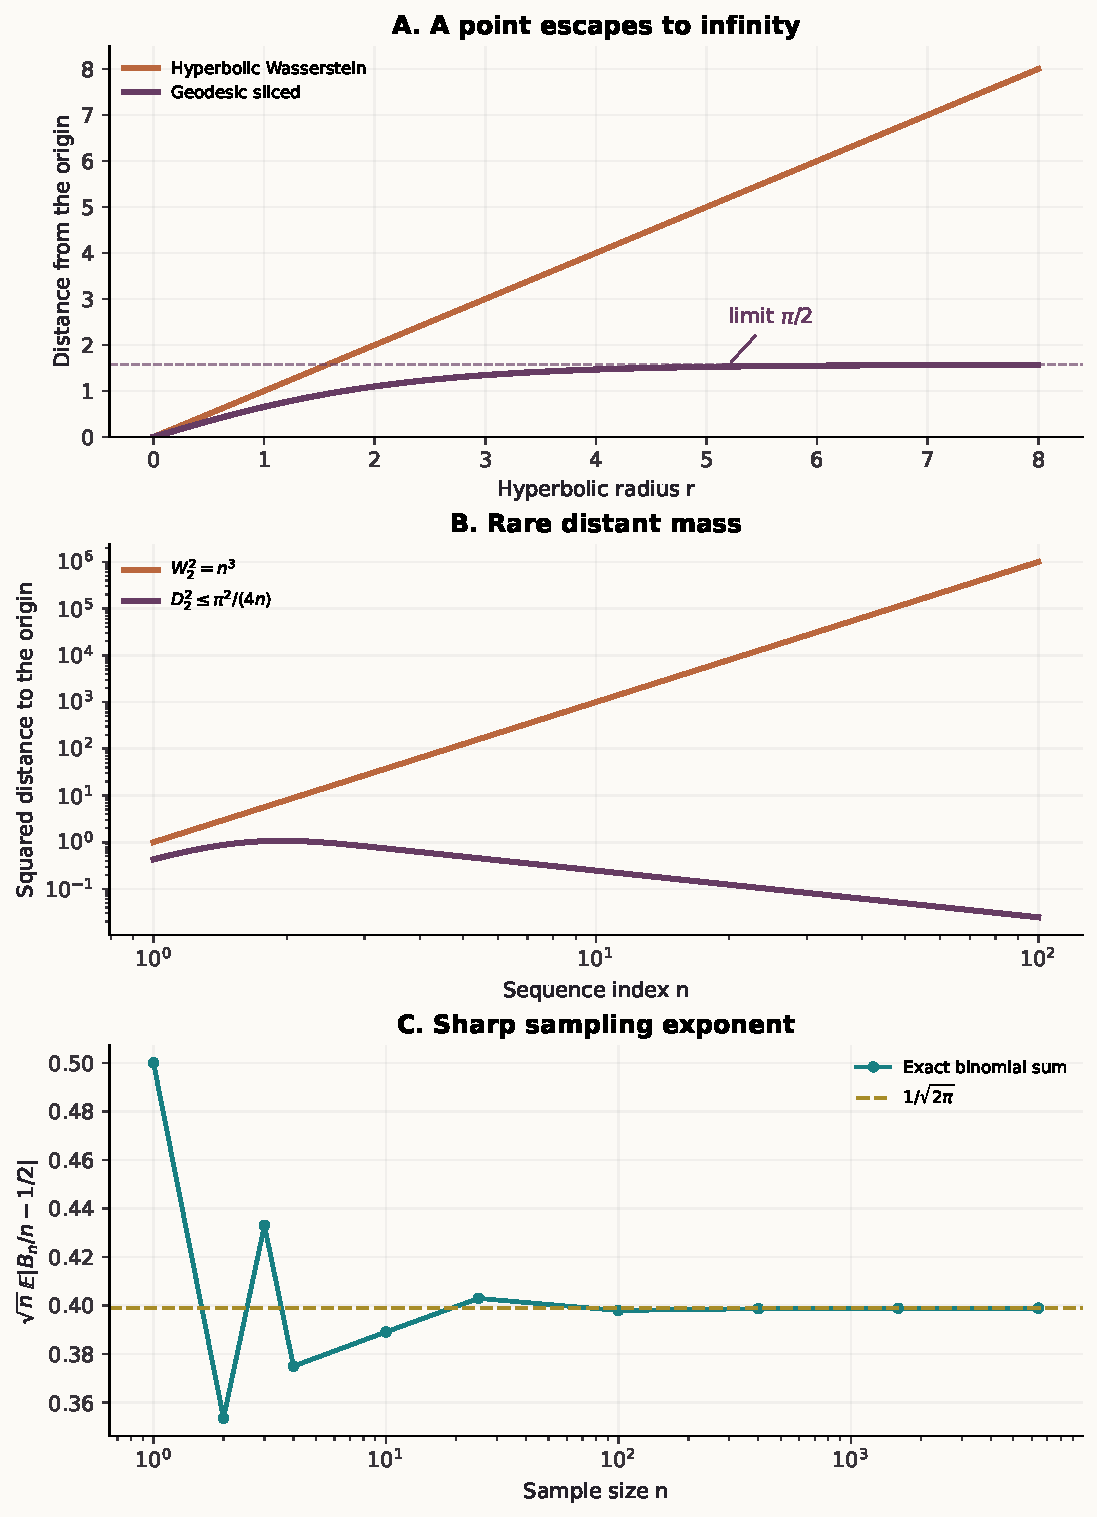
\includegraphics[width=0.9\linewidth,height=\textheight,keepaspectratio,alt={Geometry and sampling checks. Panel A compares a point mass at radius r with the origin (d=2, p=2). Panel B uses the sequence (4.1) with p=2. Panel C evaluates the exact binomial imbalance (5.6); parity explains the small alternation.}]{figures/geometry_and_sampling.pdf}
\caption{Geometry and sampling checks. Panel A compares a point mass at
radius \(r\) with the origin (\(d=2\), \(p=2\)). Panel B uses the
sequence (4.1) with \(p=2\). Panel C evaluates the exact binomial
imbalance (5.6); parity explains the small alternation.}
\end{figure}

\begin{figure}
\centering
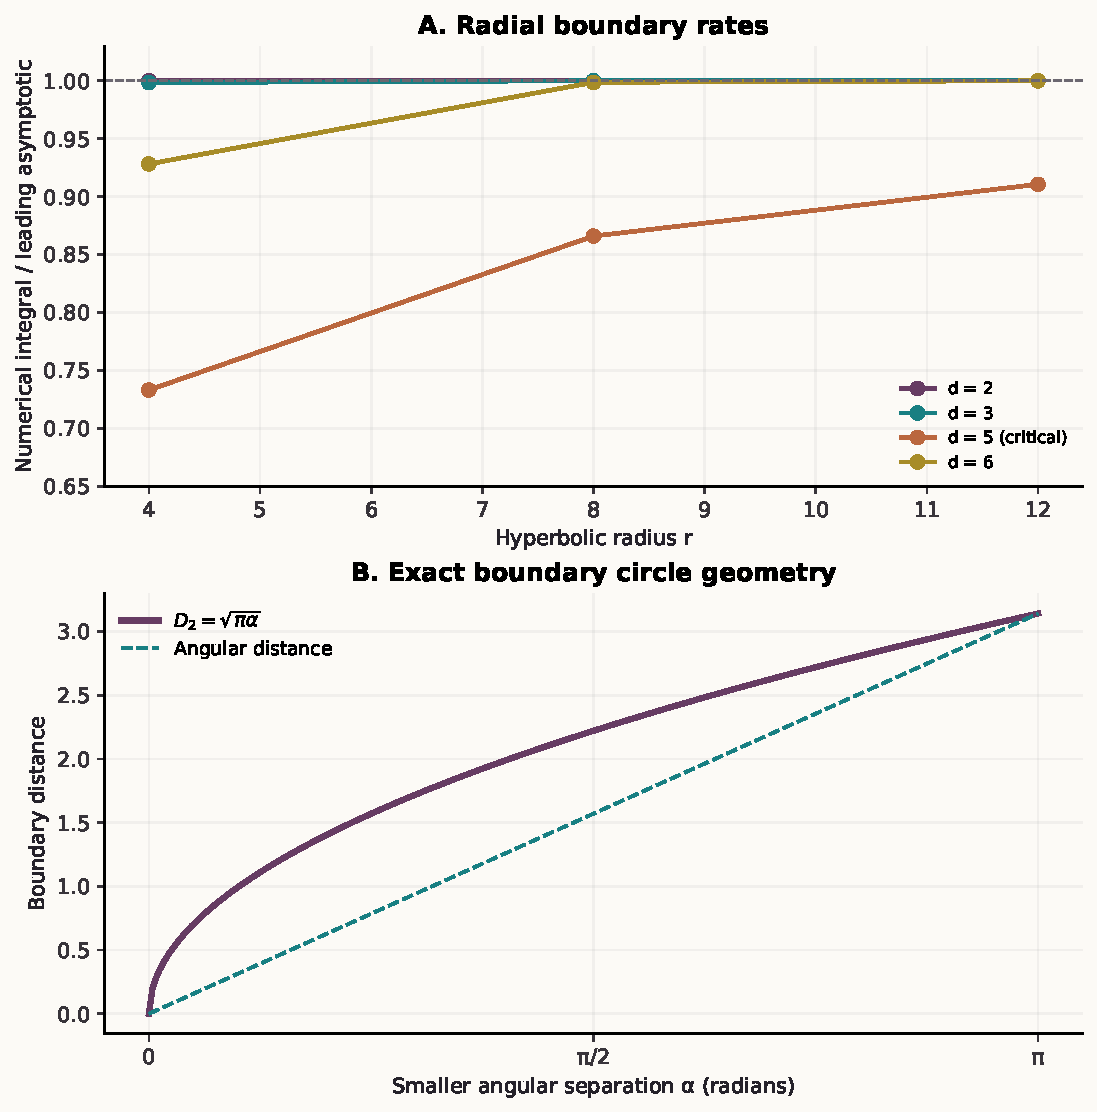
\includegraphics[width=0.9\linewidth,height=\textheight,keepaspectratio,alt={Boundary checks for quadratic loss. Panel A divides (4.5) by its leading asymptotic; the critical dimension d=5 converges more slowly. Panel B shows the boundary metric (4.9) for d=2; the dashed angular distance is a reference only.}]{figures/boundary_rates.pdf}
\caption{Boundary checks for quadratic loss. Panel A divides (4.5) by
its leading asymptotic; the critical dimension \(d=5\) converges more
slowly. Panel B shows the boundary metric (4.9) for \(d=2\); the dashed
angular distance is a reference only.}
\end{figure}

\textbf{Limits.} The theorems concern real hyperbolic space, a fixed
origin, the uniform angular measure, \(d\geq2\) and finite \(p\).
Changing the origin changes the metric (by an isometry of the whole
picture), so results hold for each fixed origin but data-dependent
origins are not covered. Other angular measures, the horospherical
construction, general Cartan--Hadamard manifolds, sharp minimax
constants and sampling rates for the augmented metric remain open.

\textbf{Status.} This is an unrefereed candidate. It has had AI-assisted
review (five simulated reviewers, an independent adversarial review and
a clean replay of the code), not external human peer review or formal
verification. The literature search is bounded and cannot certify
priority. This version (0.1.0-candidate) is archived at Zenodo with DOI
\href{https://doi.org/10.5281/zenodo.23938270}{10.5281/zenodo.23938270}
(all versions:
\href{https://doi.org/10.5281/zenodo.23938269}{10.5281/zenodo.23938269});
code and data are at
\url{https://github.com/ipitchford/hyperbolic-sliced-wasserstein-completion},
and a plain-English summary is at
\url{https://evidencepress.org/releases/hyperbolic-sliced-wasserstein-completion/}.

\section{8. Conclusion}\label{conclusion}

Geodesic hyperbolic sliced Wasserstein distance is, exactly, a metric
for weak convergence on the compact closed Klein ball. This one fact
explains its behaviour: it is bounded with an exact diameter, it sees
mass escaping to infinity as converging to the boundary, it barely
distinguishes depths far from the origin, its boundary sphere has a
dimension-dependent geometry that we computed in every dimension, and it
can be estimated at optimal distribution-free rates. Users who need
transport-moment control should add the one radial term of Theorem 6.1.
The correction to Proposition 19 of \citet{BDC2025} shows that the
vanishing-at-infinity step does not transfer from Euclidean to
hyperbolic projections.

\renewcommand\refname{References}
\bibliography{refs}

\end{document}
